\documentclass[11pt]{article}
\usepackage{amsmath,amssymb,graphicx,enumerate}
\usepackage{hyperref}
% \usepackage[parfill]{parskip}
\hypersetup{
    colorlinks=true,
    linkcolor=blue,
    filecolor=magenta,      
    urlcolor=blue,
}

\def\Homework{5} % Number of Homework
\def\Session{Spring 2022}
\def\Section{B}
\def\MyEmail{husam.almanakly@cooper.edu}

\title{MATLAB Assignment \Homework}
\author{\Session, Section \Section}
\date{March 9th, 2022}

\newenvironment{qparts}{\begin{enumerate}[{(}a{)}]}{\end{enumerate}}

\textheight=9in
\textwidth=6.5in
\topmargin=-.75in
\oddsidemargin=0.25in
\evensidemargin=0.25in


\begin{document}

\maketitle
    
    \noindent
 In this homework, we're going to go through a few data structures that we covered in class like structures, classes, and chars. We will also go through file input and output in MATLAB. You will need to import in a kickstarter project statistic from \url{https://www.kaggle.com/socathie/kickstarter-project-statistics} and encapsulating it in classes. After obtaining all the data, you will be required to write some funtions for the class you just created. It is advised that after each stage, you save your variables, say, all your kickstarter instances, into a .mat file such that you would not need recreate all the classes again.
 
 \bigskip
 \noindent \textbf{1.} First, create a class called kickstarter. In your kickstarter class, you should have the following properties. Note that you do not need to specify the data type of the properties when you are declaring a class – the following properties are just here to impress on you what type of properties you would be expecting
 \begin{itemize}
    \item amtpledged : Double
    \item by : Char
    \item category : Char
    \item currency : Char
    \item goal : Double
    \item City : Char
    \item State : Char
    \item numbackers : Double
    \item pledgetier : A struct with the fields pledge and numbackers, which store the pledge amount and the number of backers of that pledge. Note in the dataset, these two fields of the struct are labelled pledgetier and numbackerstier. 
    \item title : Char
    \item url : Char
 \end{itemize}
 
 
 \bigskip
 \noindent \textbf{2.} Now, import the data from \emph{most\_backed.csv} into MATLAB and store it in a cell array of kickstarter instances (go to the above link and download the file named most\_backed.csv, and put it in the same directory as your project). You're going to want to use a for loop to create every instance of kickstarter and store it in the cell array. Make sure that the properties of kickstarter are the datatype listed above! Note that in the dataset, the city and the state are in the same char. You would need to split the char first before you assign City and State to your values.
 
 \bigskip
 \noindent \textbf{3.} In your kickstarter class, create a function called \emph{plotTiers} which plots a bar chart of the number of tiers against the number of backers for each tier. This portion is going to use the pledgetier struct that each kickstarter instance should have! Here's an example of the plot from my code plotting the data for row 38 (3Doodler title)
 
 \begin{figure}[ht]
     \centering
     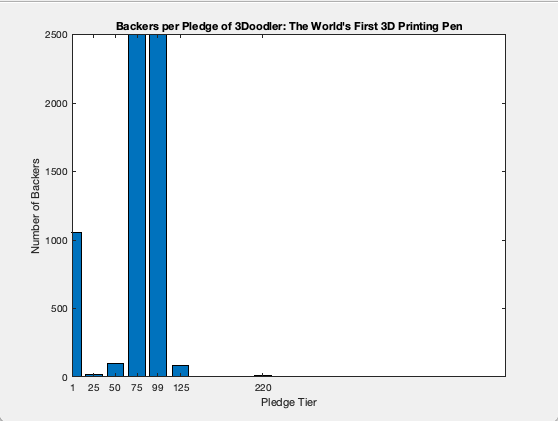
\includegraphics[width=10cm,height=10cm,keepaspectratio]{example.png}
     \caption{Example Bar Chart - Note x axis is limited from 0 - 500}
     \label{fig:my_label}
 \end{figure}
 
 \medskip
 \noindent
 One important thing to note is your function will not work on some instances of the kickstarters. The issue is with the data itself, some of the pledges will have duplicate pledge amounts (and duplicate numbackers corresponding). To fix this, find a way to remove the duplicate entries in kickstarters and numbackers before plotting the bar chart.
 
 \bigskip
 \noindent \textbf{4.} In your class, create another function called convertCurrency, which takes a char as an input. The goal of this function is to take in a char representation of a currency (’gbp’,’usd’,’eur’,’cad’) and then perform a currency conversion on all the properties in the kickstarter instance that involve money. At the end, the object should have a new currency char and all its numeric value should be converted to said currency. The following table is the currency conversion you can use for this portion:
 
 \begin{center}
     \begin{tabular}{c | c | c | c | c}
          Currency & usd & gbp & eur & cad \\ 
          \hline
          Conversion & 1 & 0.80 & 0.95 & 1.31 
     \end{tabular}
 \end{center}
 
 \bigskip
 \noindent \textbf{5.} At the end, please save your large cell array of 4000 kickstarter projects as a .mat file. Submit all your code on teams, including your script file, class file, and the .mat file you just created so that I can run your code and conduct my own tests as well! 
 
 \end{document}
